% Copyright (C) 2017 - Michael Baudin

  \documentclass{beamer}

%\setbeameroption{hide notes}
%\setbeameroption{show notes}
%\setbeameroption{show only notes}

  % Copyright (C) 2012 - EDF R&D - Michael Baudin

% To highlight source code
\usepackage{listings}
\definecolor{darkgreen}{rgb}{0,0.5,0}
\definecolor{violet}{rgb}{0.5,0,1}

\usepackage{lmodern}% http://ctan.org/pkg/lm

\usetheme{Montpellier}
\setbeamertemplate{navigation symbols}{} % Remove navigation
\useoutertheme{infolines}

\usepackage[utf8]{inputenc}
\usepackage[T1]{fontenc}

%\usepackage[french]{babel}
%\uselanguage{French}
%\languagepath{French}

\def\bx{{\bf x}}
\def\RR{\mathbb{R}}

\newcommand{\pyvar}[1]{\texttt{#1}}

\def \ot {OpenTURNS}

\hypersetup{colorlinks=true}

\usepackage{adjustbox}

\title[OpenTURNS]{OpenTURNS User day 2020}

% \author[OpenTURNS et al.]{
% Régis Lebrun, Julien Schueller
% }

% \institute[Airbus-EDF-IMACS-ONERA-Phimeca]{
% \inst{1} Airbus
% \inst{2} EDF R\&D. 6, quai Watier, 78401, Chatou Cedex - France, michael.baudin@edf.fr \and %
% \inst{3} IMACS
% \inst{4} ONERA
% \inst{5} Phimeca Engineering. 18/20 boulevard de Reuilly, 75012 Paris - France, schueller@phimeca.com
% }

\date[]{UserDay \#13, 5 June 2020, online event}
%%%%%%%%%%%%%%%%%%%%%%%%%%%%%%%%%%%%%%%%%%%%%%%%%%%%%%%%%%%%%%%%%%%%%%%%%%%%%

  \begin{document}

%%%%%%%%%%%%%%%%%%%%%%%%%%%%%%%%%%%%%%%%%%%%%%%%%%%%%%%%%%%%%%%%%%%%%%%%%%%%%

  \begin{frame}
  \titlepage

  \begin{columns}
  \begin{column}[t]{0.05\textwidth}
        \end{column}
  
    \column{0.10\textwidth}
  \begin{center}

\includegraphics[height=0.04\textheight]{figures/airbus-logo-3d-blue.png}
\end{center}

    \column{0.05\textwidth}
  \begin{center}

\includegraphics[height=0.09\textheight]{figures/logo-edf.jpg}
\end{center}

     \column{0.05\textwidth}
  \begin{center}

\includegraphics[height=0.09\textheight]{figures/imacs-logo.jpg}
\end{center}

    \column{0.10\textwidth}
  \begin{center}

\includegraphics[height=0.05\textheight]{figures/onera-logo.png}
\end{center}

    \column{0.15\textwidth}
  \begin{center}

\includegraphics[height=0.08\textheight]{figures/logo-phimeca.png}
\end{center}

\column{0.01\textwidth}

  \end{columns}

  \end{frame}

\begin{frame}
\frametitle{Session 1: 5 june 2020}


%   \begin{columns}
%     \column{0.6\textwidth}
% New features since last year in releases:
% 
\begin{itemize}
\item 9h30-10h30: "Group kernels for Gaussian process metamodels with categorical input", O. Roustant (INSA Toulouse)
\item 10h30-11h: "OpenTURNS release highlights", R. Lebrun (Airbus), J. Schueller (PhiMeca)
\item 11h-11h30: "Probabilistic analyses of a spatial vehicle equipment bay", A. Dumas (PhiMeca)
\item 11h30-12h: "Uncertainties in civil engineering: A FE-model calibration process for cultural heritage applications", VC. Kovacevic (Kobe Innovation Engineering), M. Betti (University of Florence)
\end{itemize}

% \begin{center}
% 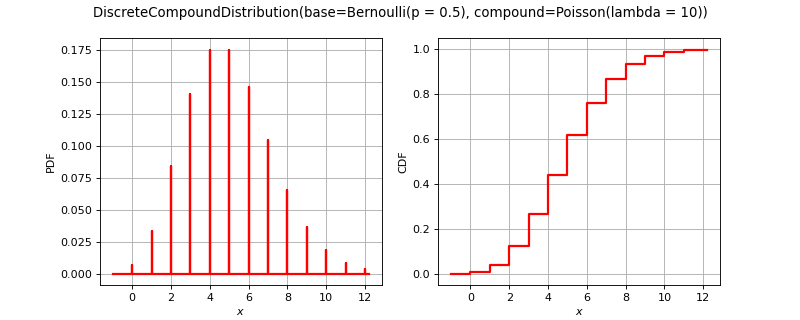
\includegraphics[width=0.8\textwidth]{figures/openturns-DiscreteCompoundDistribution-1.png}
% \end{center}
%     \column{0.4\textwidth}

% 	\begin{center}
% 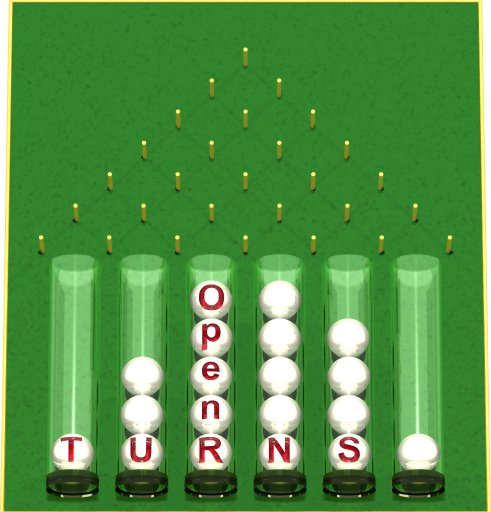
\includegraphics[width=0.9\textwidth]{figures/logo-ot}
% \end{center}

% 	\end{columns}
\end{frame}


\begin{frame}
\frametitle{Session 2: 19 june 2020}

%   \begin{columns}
%     \column{0.6\textwidth}
% New features since last year in releases:
% 
\begin{itemize}
\item 9h30-10h: "New features of Persalys', M. Baudin (EDF), J. Schueller (PhiMeca)
\item 10h-10h30: "Gaussian process approximation of a multidisciplinary system and sensitivity analysis to model uncertainty", S. Dubreuil (ONERA)
\item 10h30-11h: "Immersive and interactive scientific visualisation with Skyreal linked to OpenTURNS", H. Falgarone (Skyreal)
\item 11h-11h30: "Understanding and improvement of ingot manufacturing process using a numerical sensitivity analysis", Ch. Demay (EDF)
\item 11h30-12h: "Uncertainty quantification in hydraulics: overview of EDF applications", C. Goeury, F. Zaoui (EDF)
\end{itemize}

% \begin{center}
% 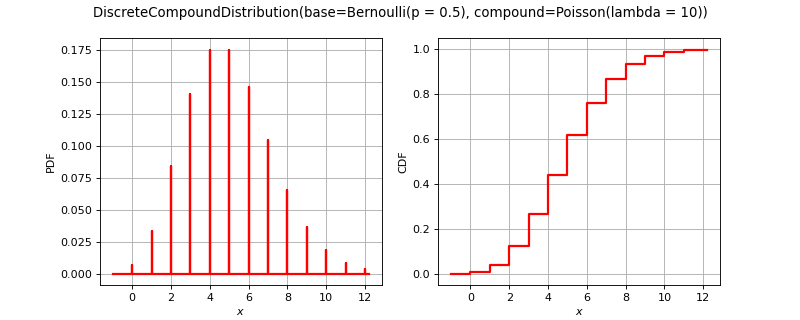
\includegraphics[width=0.8\textwidth]{figures/openturns-DiscreteCompoundDistribution-1.png}
% \end{center}
%     \column{0.4\textwidth}

% 	\begin{center}
% 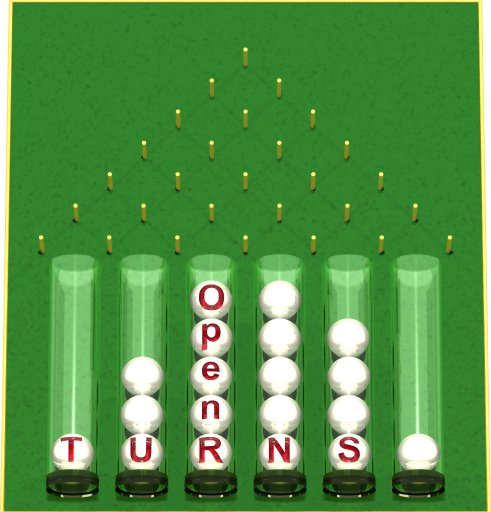
\includegraphics[width=0.9\textwidth]{figures/logo-ot}
% \end{center}

% 	\end{columns}
\end{frame}


\end{document}
